\subsection{Company Image}
%Philipp
The company image is a very important KPI to measure the company reputation. The company image is the sum of many small activities which leaves a footprint that can be recognized with the company. Single activities can improve or destroy the company image from the point of view of individuals. The goal of a high valued company image is of course monetary benefit. Therefore, activities which tend to increase the company image are not for free and it is always a difficult assessment whether to invest in a certain activity or not. In the game we concentrated on factors which can be realistically and interestingly be influenced by the player.

\begin{longtable}[]{l|c|c}
     \textbf{Action} & \textbf{Points} & \textbf{Monetary impact} \\
     \hline \hline
     \underline{\textbf{Social Engagement}} & & \\ [1ex]
     \multicolumn{1}{c|}{\textbf{CSR Donations (in \% of profit)}} & & Depending on profit \\
     No donations & 0 &  \\
     0 \% - 1 \% & 1 &  \\
     1 \% - 2 \% & 2 &   \\
     2 \% - 5 \% & 3 &   \\
     More than 5 \% & 4 &   \\ [1ex]
     \multicolumn{1}{c|}{\textbf{Support Refugee Projects}} & & \\
     Never & 0 &  \\
     1 project per year & 1 & -1000 \$ per year  \\
     2 projects per year & 2 & -2000 \$ per year   \\
     3 projects per year & 3 & -3000 \$ per year  \\
     4 projects per year & 4 & -4000 \$ per year  \\
     \hline \hline
     \underline{\textbf{Environmental Friendly Production}} & & \\ [1ex]
     \multicolumn{1}{c|}{\textbf{Supplier}} & & \\
     Eco-friendly & 2 & +10\% of cost \\
     Standard & 0 & 0\$  \\
     \multicolumn{1}{c|}{\textbf{Logistics Partner}} & & \\
     Eco-friendly & 2 & +10\% of cost \\
     Standard & 0 & 0\$  \\
     \hline \hline
     \underline{\textbf{Promotes a green image}} & & \\ [1ex]
     \multicolumn{1}{c|}{\textbf{Mandatory training for employees}} & & \\
     Never & 0 & 0 \\
     1 time per year & 1 & -1000\$ per employee  \\
     2 time per year & 2 & -2000\$ per employee  \\
     3 time per year & 3 & -3000\$ per employee  \\
     4 time per year & 4 & -4000\$ per employee  \\
     \multicolumn{1}{c|}{\textbf{Green marketing campaign}} & & \\
     Never & 0 & 0 \\
     1 time per year & 1 & -2500 \$  \\
     2 time per year & 2 & -5000 \$  \\
     3 time per year & 3 & -7500 \$  \\
     4 time per year & 4 & -10000 \$  \\
     \hline \hline
     \underline{\textbf{Promotes diversity}} & & \\ [1ex]
     \multicolumn{1}{c|}{\textbf{Mandatory diversity training}} & & \\
     Never & 0 & 0 \\
     1 time per year & 1 & -1000\$ per employee  \\
     2 time per year & 2 & -2000\$ per employee  \\
     3 time per year & 3 & -3000\$ per employee  \\
     4 time per year & 4 & -4000\$ per employee  \\
     \multicolumn{1}{c|}{\textbf{Diversity campaign}} & & \\
     Never & 0 & 0 \\
     1 time per year & 1 & -3000 \$  \\
     2 time per year & 2 & -6000 \$  \\
     3 time per year & 3 & -9000 \$  \\
     4 time per year & 4 & -12000 \$  \\
     \hline 
\caption{Actions influencing the Company Image}
    \label{tab:benefitsCIS}
\end{longtable}

The total sum of the above possible choices is the total Company Image Score (CIS). The score can reach values from 0 to 28 as it is the case for the Employee Satisfaction Score. In order to build also here a more realistic representation we figured out that the marginal benefit of an increase of the company image increases with the collected amount of points. Therefore, we manipulated also this formula and came up with the following function.

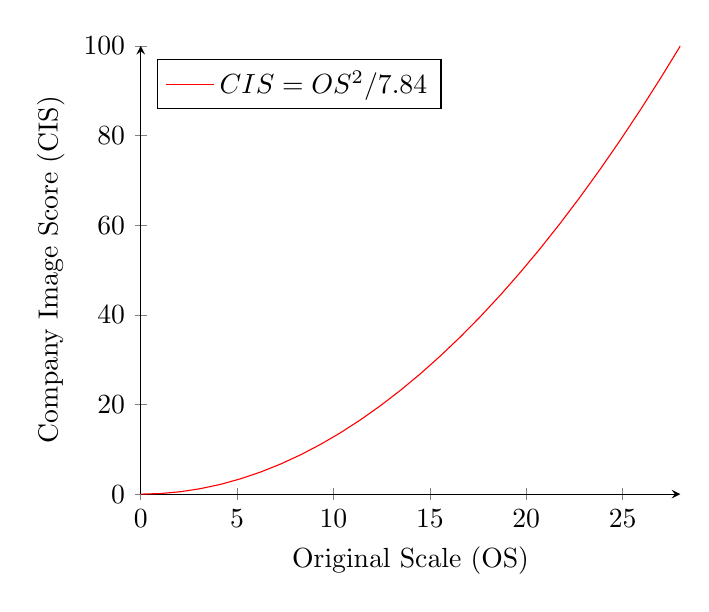
\begin{tikzpicture}
\begin{axis}[
    axis lines = left,
    xlabel = Original Scale (OS),
    ylabel = Company Image Score (CIS),
    grid style = dashed,
    legend pos=north west
]

\addplot [
    domain=0:28, 
    samples=28, 
    color=red,
]
{x^2/7.84};
\addlegendentry{$CIS=OS^2/7.84$}
\end{axis}
\end{tikzpicture}

The original scale of 0 to 28 is squared and divided by the factor of 7.84 in order to map the original scale on a scale of 0 to 100. In this case the rational behind the mapping is the fact that little activities do not have such  a big influence on the overall image of a company. When a company starts to combine all its activities it can generate huge impact and publicity which leads to a strong increase of the Company Image Score.